\documentclass{article}
\usepackage{josuamathheader}
\newcommand{\mylim}{\lim\limits_{n\to \infty}}
\usepackage{graphicx}

\begin{document}
	\analayout{6}
	\section*{Aufgabe 1}
	\begin{enumerate}[(a)]
		\item Es gilt: $\mylim \frac{3}{n} = 0$, $\mylim \frac{1}{n^2} = 0$, $\mylim \frac{81}{n^2} = 0$.
		Daher können wir folgern: 
		$$\mylim \frac{6n^2 + 3n - 1}{9n^2 - 81} = \mylim \frac{6 + \frac{3}{n} - \frac{1}{n^2}}{9 - \frac{81}{n^2}} \overset{\text{Lemma 2.5}}{=} \frac{6}{9} = \frac{2}{3}$$
		\item Behauptung $a_n = (-1)^n$.\\
		Beweis durch Fallunterscheidung
		\begin{itemize}
			\item $\exists k\in \N: n = 2k$: Dann ist $\frac{7^{2k} + (-13)^{2k}}{(-7)^{2k} + 13^{2k}} = \frac{7^{2k} + 13^{2k}}{7^{2k} + 13^{2k}} = 1 = -1^{2k}$
			\item $\exists k\in \N: n = 2k-1$: Dann ist $\frac{7^{2k-1} + (-13)^{2k-1}}{(-7)^{2k-1} + 13^{2k-1}} = \frac{7^{2k-1} - 13^{2k-1}}{-7^{2k-1} + 13^{2k-1}} = \frac{7^{2k-1} - 13^{2k-1}}{-(7^{2k-1} - 13^{2k-1})}  = -1 = -1^{2k-1}$
		\end{itemize}
		Da jede Folge genau dann konvergiert, wenn sie eine Cauchy-Folge ist, und $\forall n\in \N: |a_n -a_{n+1}| = 2$ ist, kann $a_n = (-1)^n$ nicht konvergieren.
		\item $a_n = \binom{42 n}{n^2} = \prod_{j=1}^{n^2}\frac{42n - j + 1}{j}$. Sei nun $n > 42$. Dann ist 
		$$\prod_{j=1}^{n^2}\frac{42n - j + 1}{j} = \prod_{j=1}^{42^2}\frac{42^2 - j + 1}{j} \cdot \underbrace{\frac{42^2 - (42^2 +1) + 1}{j}}_{ = 0} \cdot \prod_{j=42^2 + 2}^{n^2} \frac{42n - j + 1}{j} = 0$$
		Folglich ist $\mylim a_n = 0$.
		\item \textbf{Z.Z.:} $(2n)! > n^4 \forall n\in \N$ mit $n\geq 2$.
		\induktion{$n=2$: $(2\cdot 2)! = 24 > 16 = 2^4$}{Gelte die Behauptung für ein beliebiges, aber festes $n\in \N$ mit $n \geq 2$.}{$n\to n+1$
		$$(2n+2)! = (2n+2) \cdot (2n+1) \cdot (2n)! \overset{\text{I.V.}}{>} (2n+2)(2n+1)\cdot n^4 \overset{n\geq 2}{\geq} 30n^4 > n^4 + 4n^3 + 6n^2 + 4n + 1 = (n+1)^4$$}
		Daraus folgt $a_n = \frac{n^3}{\binom{2n}{n}} = \frac{n^3}{\frac{(2n)! \cdot n!}{(2n-n)!}} = \frac{n^3}{(2n)!} \leq \frac{n^3}{n^4} = \frac{1}{n}$ und $\mylim a_n = 0$.
		\item Es gilt
		$$a_n = \prod_{k=2}^{n} \left(1-\frac{1}{k}\right) = \prod_{k=2}^{n} \left(\frac{k-1}{k}\right) \overset{\text{Teleskopprodukt}}{=} \frac{1}{n}$$ und daher $\mylim a_n = 0$.
		\item Es gilt $\mylim \frac{2\sin(n)}{n} = \mylim 2\sin(n) \cdot \frac{1}{n} \overset{\text{Lemma 2.5}}{=} 0$, $\mylim \frac{1}{n} = 0$ und daher insgesamt
		$$\mylim a_n = \mylim \frac{\pi n + 2 \sin(n)}{2n + 1} = \mylim \frac{\pi + \frac{2\sin(n)}{n}}{2 + \frac{1}{n}} \overset{\text{Lemma 2.5}}{=} \frac{\pi}{2}$$
		\item Nach Vorlesung gilt (siehe Abbildung~\ref{anaskript1}): $\mylim \sqrt[n]{x^n + y^n} = \max(x,y)$
		\begin{figure}
			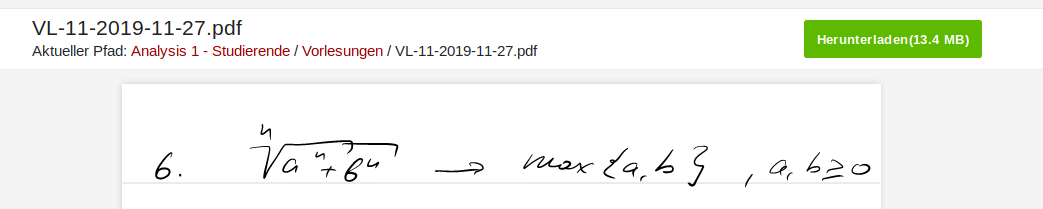
\includegraphics[width = \textwidth]{anaskript.png}
			\caption{Skript zur Analysis 1 Vorlesung vom 27.11.}
			\label{anaskript1}
		\end{figure}
		\item Es gilt
		$$n^n = \prod_{k=1}^{n}n = n\prod_{k=2}^{n}n > n\prod_{k=2}^{n}k = n \cdot n!$$
		Daraus folgt $a_n = \frac{n^n}{n!} \geq \frac{n\cdot n!}{n!} = n$. Daher ist $a_n$ nicht konvergent.
		\item Es gilt
		$$n^n\cdot n = n^2\cdot \prod_{k=1}^{n-1}n <  n^2\prod_{k=1}^{n-1}k(n+k) < n\cdot (n+n) \prod_{k=1}^{n-1}k(n+k) < \prod_{k=1}^{n}k(n+k)= \prod_{k=1}^{2n}k = (2n)!$$
		Folglich ist $a_n = \frac{n^n}{(2n)!} \leq \frac{n^n}{n^n\cdot n} = \frac{1}{n}$ und da alle $a_n> 0$ sind, gilt nach Sandwichlemma $\mylim a_n = 0$
	\end{enumerate}
	\section*{Aufgabe 2}
	Sei $s$ eine obere Schranke für $|b_n|$. Dann gilt $\forall n\in \N: 0  \leq |a_n|\cdot |b_n| \leq |a_n|\cdot s$. Da $a_n$ eine Nullfolge ist, folgt mit Lemmma 2.5 und dem Sandwichlemma sofort $\mylim |a_n|\cdot |b_n| = 0$. Ist $|a_n| \cdot |b_n| = |a_n\cdot b_n|$ eine Nullfolge, so ist offensichtlich auch $a_n\cdot b_n$ eine Nullfolge.
	\section*{Aufgabe 3}
	Sei $\mylim a_n = \mylim b_n = s\in \R$ und $\varepsilon > 0$. Dann
	$$\exists N_a\in \N: \forall n\geq N_a:|a_n-s| < \varepsilon$$ und
	$$\exists N_b\in \N: \forall n\geq N_b:|b_n-s| < \varepsilon.$$
	Folglich ist
	$$\forall n > \max(N_a, N_b): |a_n-s|< \varepsilon \text{ und } |b_n-s| <\varepsilon$$ und äquivalent dazu
	$$\forall n > \max(N_a, N_b): |c_{2n-1}-s|< \varepsilon \text{ und } |c_{2n}-s| <\varepsilon.$$
	Zusammengenommen erhalten wir
	$$\forall n\geq \max(N_a, N_b): |c_n-s|< \varepsilon.$$
	Das impliziert sofort $\mylim c_n = s$.\\
	Sei nun andererseits $\varepsilon > 0$ und $\mylim c_n = s\in \R$.
	Dann $$\exists N_c\in \N: \forall n\geq N_c: |c_n-s|< \varepsilon$$ und insbesondere gilt nun $$\forall n\geq N_c: |c_{2n}-s|< \varepsilon\text{ und }|c_{2n-1}-s| < \varepsilon.$$ Äquivalent dazu erhalten wir
	$$\forall n\geq N_c: |a_n-s|< \varepsilon \text{ und } |b_n-s|<\epsilon.$$
	Das impliziert sofort $\mylim a_n = s$ und $\mylim b_n = s$.
	\section*{Aufgabe 4}
	\begin{enumerate}[(a)]
		\item \text{Z.Z.:} $1$ und $-1$ sind die einzigen Häufungspunkte und damit $\limsup\limits_{n\to \infty} a_n = 1$ und $\liminf\limits_{n\to \infty} a_n = -1$
		\begin{proof}
			Wir betrachten 2 Teilfolgen $d_n := a_{2n-1}$ und $e_n := a_{2n}$ von $a_n$. Es gilt $d_n = \frac{(-1)^{2n}}{1 + \left(\frac{1}{2n}\right)} = \frac{1}{1 + \left(\frac{1}{2n}\right)}$ und $e_n = \frac{(-1)^{2n-1}}{1 + \left(\frac{1}{2n-1}\right)} = -\frac{1}{1 + \left(\frac{1}{2n-1}\right)}$. Mit Lemma 2.5 erhalten wir sofort $\mylim d_n = 1$ und $\mylim e_n = -1$. Daher sind $1$ und $-1$ Häufungspunkte von $a_n$. Sei $1\neq f\neq -1$ ein weiterer Häufungspunkt von $a_n$. Dann existiert eine Teilfolge $f_n$ mit $\mylim f_n = f$. Daher muss es aber auch eine Teilfolge von $d_n$ oder $e_n$ geben, die gegen $f$ konvergiert. Jede Teilfolge von $d_n$ konvergiert aber gegen $1$ und jede Teilfolge von $e_n$ konvergiert gegen $-1$. Daher ist $f = 1$ oder $f= -1$ und daher sind $1$ und $-1$ die einzigen Häufungswerte von $a_n$.
		\end{proof}
		\item \text{Z.Z.:} $1$, $0$ und $-1$ sind die einzigen Häufungspunkte und damit $\limsup\limits_{n\to \infty} b_n = 1$ und $\liminf\limits_{n\to \infty} b_n = -1$.
		\begin{proof}
			Wir definieren wieder mehrere Teilfolgen.
			Sei $g_n \coloneqq b_{10n}$, $h_n \coloneqq b_{2n-1}$ und $i_n$ die Folge aller $a_{2n}$ mit $5 \nmid n$.
			Dann ist offensichtlich $\mylim g_n = 0$.
			Mit Lemma 2.5 ist $\mylim h_n = \mylim \frac{(-1)^{2n-1}(2n)^2 + 2}{(2n+2)^2} = \mylim \frac{-4n^2 + 2}{4n^2 + 4n + 4} = \mylim \frac{-4 + \frac{2}{n^2}}{4 + \frac{4}{n} + \frac{4}{n^2}} = -1$ und $\mylim i_n = \mylim \frac{(-1)^{2n}(2n)^2 + 2}{(2n+2)^2} = \mylim \frac{4n^2 + 2}{4n^2 + 4n + 4} = \mylim \frac{4 + \frac{2}{n^2}}{4 + \frac{4}{n} + \frac{4}{n^2}} = 1$. Analog zur (a) folgt nun, dass $1$, $0$ und $-1$ die einzigen Häufungswerte unserer Folge sind und daher $\limsup\limits_{n\to \infty} b_n = 1$ sowie $\liminf\limits_{n\to \infty} b_n = -1$.
		\end{proof}
		\item \text{Z.Z.:} $\frac{5}{6}$, $\frac{1}{6}$, $-\frac{1}{6}$ und $-\frac{5}{6}$ sind die einzigen Häufungspunkte und damit $\limsup\limits_{n\to \infty} c_n = \frac{5}{6}$ und $\liminf\limits_{n\to \infty} c_n = -\frac{5}{6}$.
		\begin{proof}
			\textbf{Behauptung:}
			$$c_n = \begin{cases}
			\hfill \frac{5}{6} &| \exists k\in \N: n = 4k\\
			-\frac{5}{6} &| \exists k\in \N: n = 4k + 1\\
			\hfill\frac{1}{6} &| \exists k\in \N: n = 4k + 2\\
			-\frac{1}{6} &| \exists k\in \N: n = 4k + 3
			\end{cases}$$
			Beweis der Behauptung durch Fallunterscheidung:
			\begin{itemize}
				\item $\exists k\in \N: n = 4k$\\
				Dann ist $c_n = c_{4k} = \frac{(-1)^{4k}}{2} + \frac{(-1)^{\frac{4k(4k+1)}{2}}}{3} = \frac{1}{2} + \frac{(-1)^{2k(4k+1)}}{3} = \frac{1}{2} + \frac{1}{3} = \frac{5}{6}$.
				\item $\exists k\in \N: n = 4k + 1$\\
				Dann ist $c_n = c_{4k+1} = \frac{(-1)^{4k+1}}{2} + \frac{(-1)^{\frac{(4k+1)(4k+2)}{2}}}{3} = -\frac{1}{2} + \frac{(-1)^{(4k+1)(2k+1)}}{3} = -\frac{1}{2} - \frac{1}{3} = -\frac{5}{6}$.
				\item $\exists k\in \N: n = 4k + 2$\\
				Dann ist $c_n = c_{4k+2} = \frac{(-1)^{4k+2}}{2} + \frac{(-1)^{\frac{(4k+2)(4k+3)}{2}}}{3} = \frac{1}{2} + \frac{(-1)^{(2k+1)(4k+3)}}{3} = \frac{1}{2} - \frac{1}{3} = \frac{1}{6}$.
				\item $\exists k\in \N: n = 4k + 1$\\
				Dann ist $c_n = c_{4k+3} = \frac{(-1)^{4k+3}}{2} + \frac{(-1)^{\frac{(4k+3)(4k+4)}{2}}}{3} = -\frac{1}{2} + \frac{(-1)^{(4k+3)(2k+2)}}{3} = -\frac{1}{2} + \frac{1}{3} = -\frac{1}{6}$.
			\end{itemize}
		Die Folge nimmt also nur vier verschiedene Werte an, allerdings jeden davon unendlich oft. Daher sind $\frac{5}{6}$, $\frac{1}{6}$, $-\frac{1}{6}$ und $-\frac{5}{6}$ alle Häufungspunkte von $a_n$ und folglich ist $\limsup\limits_{n\to \infty} c_n = \frac{5}{6}$ und $\liminf\limits_{n\to \infty} c_n = -\frac{5}{6}$.
		\end{proof}
	\end{enumerate}
\end{document}